\documentclass[12pt,border=9pt]{standalone}
\usepackage[T1]{fontenc}\usepackage{lmodern}\usepackage{amsmath,amssymb}
\usepackage{tikz}\usepackage{quantikz}
\usetikzlibrary{arrows.meta,positioning,fit,calc}
\definecolor{inkPrim}{HTML}{1B1B1B}\definecolor{inkMute}{HTML}{6E6E6E}
\definecolor{coral}{HTML}{D55E00}\definecolor{blue}{HTML}{0072B2}
\definecolor{clbox}{HTML}{EAF1F7}\definecolor{spbox}{HTML}{F5EFE7}\definecolor{colbox}{HTML}{EAF3EE}
\begin{document}
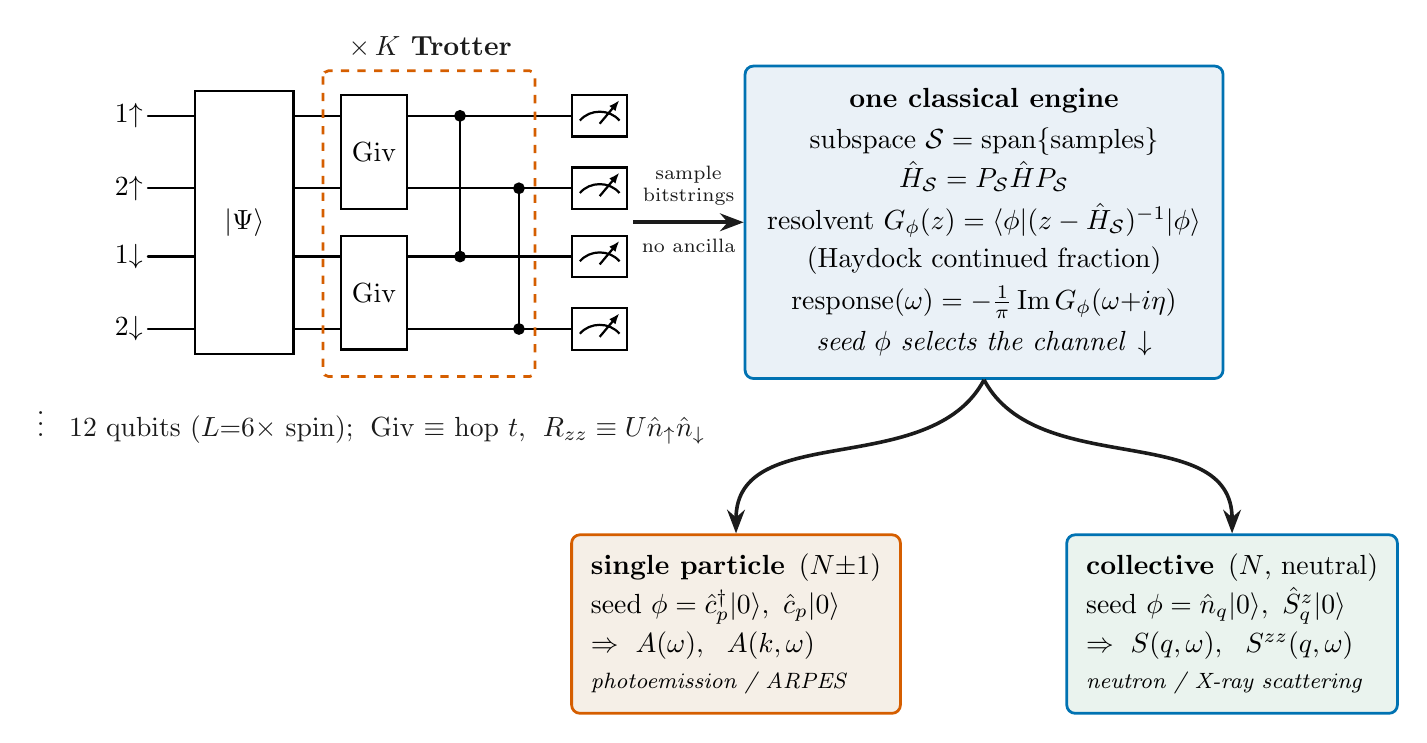
\begin{tikzpicture}[font=\rmfamily,
  arr/.style={-{Stealth[length=3mm]},line width=1.3pt,inkPrim}]
% ===================== TOP ROW: quantum sampling primitive -> one classical engine =====================
\node[inner sep=1pt] (circ) at (0,0) {%
\begin{quantikz}[row sep=0.34cm,column sep=0.60cm]
\lstick{$1{\uparrow}$} & \gate[4][1.25cm]{\lvert\Psi\rangle} & \gate[2]{\text{Giv}} & \ctrl{2} & \qw & \meter{} \\
\lstick{$2{\uparrow}$} & & & \qw & \ctrl{2} & \meter{} \\
\lstick{$1{\downarrow}$} & & \gate[2]{\text{Giv}} & \control{} & \qw & \meter{} \\
\lstick{$2{\downarrow}$} & & & \qw & \control{} & \meter{}
\end{quantikz}};
\node[inkPrim,font=\normalsize\bfseries,anchor=south] at ([yshift=6pt,xshift=0.75cm]circ.north) {$\times\,K$ Trotter};
\draw[coral,line width=1.0pt,dashed,rounded corners=2pt]
  ([xshift=2.72cm,yshift=5pt]circ.north west) rectangle ([xshift=-1.25cm,yshift=-6pt]circ.south east);
\node[font=\normalsize,inkPrim,anchor=north] at ([yshift=-9pt]circ.south)
  {$\vdots$\;\; $12$ qubits ($L{=}6\times$ spin);\; Giv $\equiv$ hop $t$,\; $R_{zz}\equiv U\hat n_\uparrow\hat n_\downarrow$};
% one classical engine (top-right)
\node[draw=blue,fill=clbox,rounded corners=3pt,line width=1.0pt,inner sep=8pt,align=center,font=\normalsize,
      right=1.4cm of circ] (eng)
  {\textbf{one classical engine}\\[3pt]
   subspace $\mathcal S=\mathrm{span}\{\text{samples}\}$\\[2pt]
   $\hat H_{\mathcal S}=P_{\mathcal S}\hat H P_{\mathcal S}$\\[3pt]
   resolvent $G_\phi(z)=\langle\phi|(z-\hat H_{\mathcal S})^{-1}|\phi\rangle$\\[2pt]
   (Haydock continued fraction)\\[3pt]
   $\text{response}(\omega)=-\tfrac1\pi\,\mathrm{Im}\,G_\phi(\omega{+}i\eta)$\\[3pt]
   {\itshape seed $\phi$ selects the channel}\, $\downarrow$};
\draw[arr] (circ.east) -- node[above=2pt,font=\scriptsize,inkPrim,align=center]{sample\\bitstrings}
                            node[below=2pt,font=\scriptsize,inkPrim]{no ancilla} (eng.west);
% ===================== BOTTOM ROW: one primitive -> four dynamical responses =====================
\node[draw=coral,fill=spbox,rounded corners=3pt,line width=1.0pt,inner sep=7pt,align=left,font=\normalsize,anchor=north]
      (sp) at ([xshift=-3.15cm,yshift=-1.95cm]eng.south)
  {\textbf{single particle}\, ($N{\pm}1$)\\[2pt]
   seed $\phi=\hat c^\dagger_p\lvert0\rangle,\ \hat c_p\lvert0\rangle$\\[2pt]
   $\Rightarrow\ A(\omega),\ \ A(k,\omega)$\\[1pt]
   {\footnotesize\itshape photoemission / ARPES}};
\node[draw=blue,fill=colbox,rounded corners=3pt,line width=1.0pt,inner sep=7pt,align=left,font=\normalsize,anchor=north]
      (col) at ([xshift=3.15cm,yshift=-1.95cm]eng.south)
  {\textbf{collective}\, ($N$, neutral)\\[2pt]
   seed $\phi=\hat n_q\lvert0\rangle,\ \hat S^z_q\lvert0\rangle$\\[2pt]
   $\Rightarrow\ S(q,\omega),\ \ S^{zz}(q,\omega)$\\[1pt]
   {\footnotesize\itshape neutron / X-ray scattering}};
% fan-down arrows: same engine + subspace, seed phi picks the channel
\draw[arr] (eng.south) to[out=-118,in=90] (sp.north);
\draw[arr] (eng.south) to[out=-62,in=90] (col.north);
\end{tikzpicture}
\end{document}
